\typeout{NT FILE chapter4.tex}%

\chapter{Work Done}
\label{Work Done}

In this chapter we will discuss all the work already done by now to enhance the software quality of the application.

\section{Main Contributions}

One of my key responsibilities is the analysis of the modules Profiles and Notifications. This involves a deep review of requirements and the creation of alternative representation models to enhance the understanding.

I am currently creating a specification of the application profiles and permissions using a new organizational matrix. This significantly helped us to see where code could be factorised during our further developments. Ensuring precise permissions is crucial for maintaining both security and functionality.

Additionally, I am enhancing our version control practices by implementing GIT. I have documented this methodology to ensure its effectiveness. Furthermore, I am leading our team through the transition to this new system, ensuring a smooth adoption. Our progress includes phases such as code cleanup, repository setup, script variabilization and training.

In collaboration with stakeholders, I am actively involved in the development of new features and integrations across various technologies, including PowerShell, C, XML, JSON, and SQL. Upcoming major projects include the integration of the L684 SAS Server application (manual + AD provisioning) and the L716-SIMPLISSIMO application (manual provisioning).

\section{Refactoring the Codebase}

\subsection{Application Profiles}

One of the main tasks was to understand how the Usercube application manages the restrictions within the application configuration and then to fix the known issues. The first step was to analyse in the codebase what was all the configuration elements that was connected with the profiles declaration and then to review the definition of each of these elements in the Usercube documentation ~\cite{UsercubeDocument}.

\begin{figure}
    \centering
    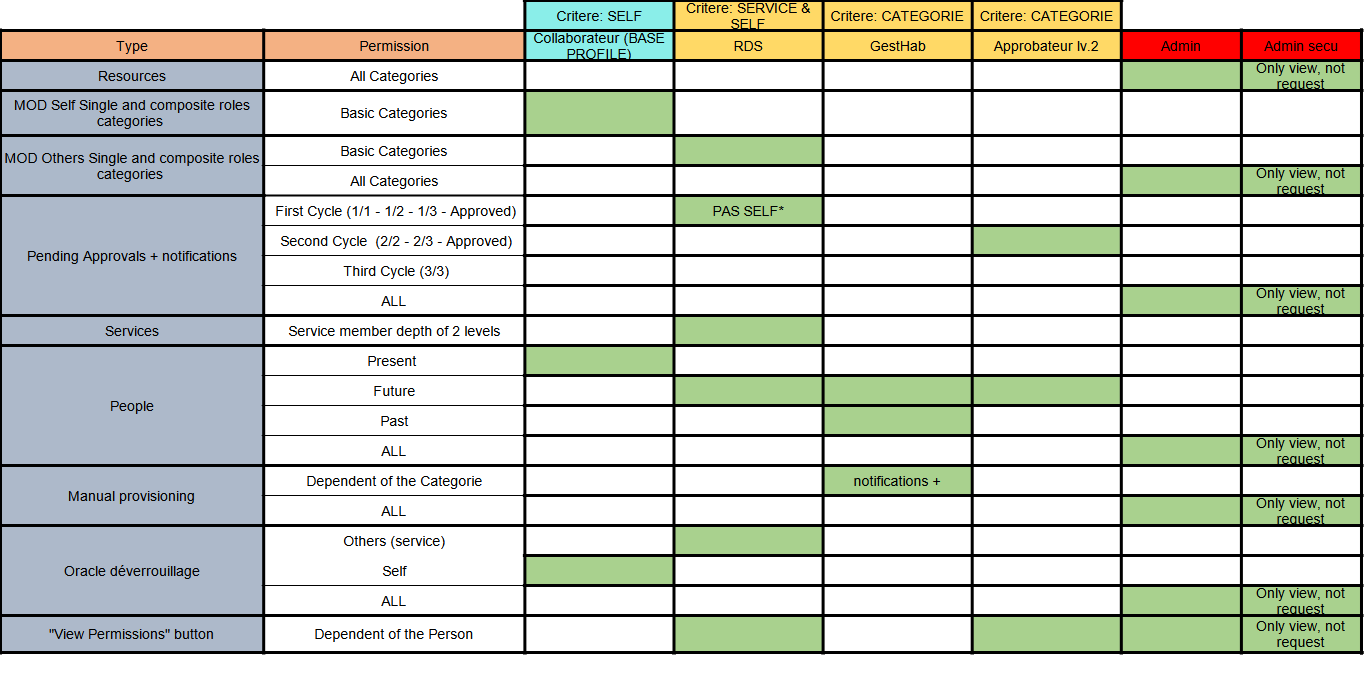
\includegraphics[width=1\linewidth]{profilsAna.png}
    \caption{Table with definition of profiles}
    \label{fig:enter-label}
\end{figure}

The table was the most important thing to ensure the effective communication with the Team in France responsable for the projetct. Before this unique table with all the profiles next to the other for better comparison we had an excel file with long pages and description wrote by the QA team previously when the profiles were asked in the origin of it. The table was only possible trough understanding the steps of our workflows and what is the true concerning of each profile.

\begin{table}[h]
    \centering
    \begin{tabular}{lcc}
        \toprule
        & \textbf{Old Version} & \textbf{New Version} \\
        \midrule
        Lines of Code & 4698 & 1807 \\
        \midrule
        Entry Elements & 1127 & 350 \\
        Filter Elements & 1181 & 606 \\
        AccessControlRule Elements & 616 & 188 \\
        \quad Related to EntityType="SingleRole" & 52 & 4 \\
        \quad Related to EntityType="Category" & 54 & 4 \\
        \quad Related to EntityType="ResourceType" & 51 & 4 \\
        \bottomrule
    \end{tabular}
    \caption{Comparison of Old and New Versions}
    \label{tab:comparison}
\end{table}

The new version of the code has been significantly reduced, decreasing the total lines of code from 4698 to 1807. This includes a reduction in the number of elements for "entry" from 1127 to 350, "filter" from 1181 to 606, and "AccessControlRule" from 616 to 188. The "AccessControlRule" elements related to "SingleRole," "Category," and "ResourceType" have all been reduced from around 50 each to just 4. This substantial simplification suggests a more efficient and maintainable codebase.

\subsection{Notifications}

The notifications are a very important aspect of the Usercube application since it is the way the managers responsibles for approving the demands of permissions are notified. The Notifications are directly related to the profiles. The application uses the same Entry permission mechanism to attach which profiles are going to be notified depending on the case.

Since the profiles had many problems the team always had a big trouble making sure the right person receive the right notification. Immediatly after deploying the profiles to quality we started digging into the notifications scripts in PowerShell that were created in order to substitute the native ones.

\section{Implementing Version Control with Git}

The process began with the creation of the main production branch. From there, a pre-production branch (PKG-V24S23) was derived, followed by a QA branch (REC-V24S23). These branches ensured that code progressed through stages of preparation and quality assurance before reaching production. Feature and fix branches, such as feat/Mantis-XXXXX and fix/Mantis-YYYYY, were created for specific tasks and issues, allowing focused development and bug fixing. These branches were periodically merged back into the QA branch and pre-production branch, ensuring continuous integration and testing. Eventually, all changes were merged into the main production branch, culminating in stable release tags like V24S23 and V24S27. This structured approach promoted organized development, thorough testing, and smooth integration of new features and fixes.

\begin{figure}
    \centering
    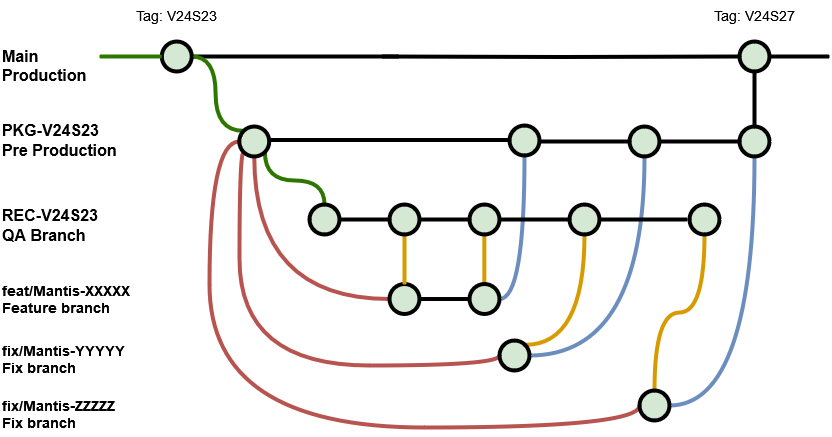
\includegraphics[width=1\linewidth]{GitDiagram.png}
    \caption{Git Branching Diagram}
    \label{fig:git-diagram}
\end{figure}

Version control is indispensable for managing collaborative software development. Our phased approach to implementing Git involved preparatory activities such as code cleanup and repository setup. Further steps included script variabilization and adaptation for diverse environments, culminating in team training to foster proficient utilization of the version control system.

\section{Integrations and New Features}

The applications Mantis de recette, ORP WEB, Tables START, SIMPLISSIMO and SAS Serveur were integrated into AnA and are now managed by the system. 

Integrating a new application consists in connecting a system, automatically via Active Direchetorie or manually via csv files. Newer applications that are alreading doing the authorization via AD can be fully automated by usercube, older one depends on keeping track of 2 csv files: one that mantaings a record of all the roles possible for the application and another containing the attribuition of these roles.

The integration is done by adding the references of the application to be integrated in the xml code using the elements designed to create connectors. Connectors are how these connections are called.